% *****************************************************************************************************
% ****************************              SIMPLE EXAMPLE             ********************************
% *****************************************************************************************************

% =======================================================
% =======         HEADER FOR DOCUMENT        ============
% =======================================================
    
    % *********  SPECIFIC FOR THIS BOOK  ********
    \def\ProjectAuthorLink{https://github.com/CompilandoConocimiento}
    \def\ProjectNameLink{\ProjectAuthorLink/LibroProbabilidad}    
    

    % *********   DOCUMENT ITSELF   **************
    \documentclass[fleqn, journal]{IEEEtran}                        %Type of doc and size of font and left equations
    \usepackage{ifthen}                                             %Allow simple programming using if - then
    \usepackage[hidelinks]{hyperref}                                %Allow to create hiperlinks and Fuck Firefox
    \usepackage{pdfpages}                                           %Allow us 'import' PDF's
    \hypersetup{pageanchor=false}                                   %Solve 'double page 1' warnings in build :v
    \setlength{\parindent}{0pt}                                     %Eliminate ugly indentation
    \author{Oscar Andrés Rosas}                                     %Who I am

    % *********   LANGUAJE    *****************
    \usepackage[spanish]{babel}                                     %Please allow me to type in spanish
    \usepackage[utf8]{inputenc}                                     %Lets use UFT-8
    \usepackage[T1]{fontenc}                                        %Allow for better font support
    \usepackage{textcmds}                                           %Allow us to use quoutes
    \usepackage{changepage}                                         %Allow us to use identate paragraphs
    \usepackage{anyfontsize}                                        %All the sizes for fonts wiiiii!

    % *********   MATH AND HIS STYLE  *********
    \usepackage{ntheorem, amsmath, amssymb, amsfonts}               %All fucking math, I want all!
    \usepackage{mathrsfs, mathtools, empheq}                        %All fucking math, I want all!
    \usepackage{cancel}                                             %Negate symbol
    \usepackage{centernot}                                          %Allow me to negate a symbol
    \decimalpoint                                                   %Use decimal point

    % *********   GRAPHICS AND IMAGES *********
    \usepackage{graphicx}                                           %Allow to create graphics
    \usepackage{float}                                              %For images
    \usepackage{wrapfig}                                            %Allow to create images
    \graphicspath{ {Graphics/} }                                    %Where are the images :D

    % *********   LISTS AND TABLES ***********
    \usepackage{listings, listingsutf8}                             %We will be using code here
    \usepackage[inline]{enumitem}                                   %We will need to enumarate
    \usepackage{tasks}                                              %Horizontal lists
    \usepackage{longtable}                                          %Lets make tables awesome
    \usepackage{booktabs}                                           %Lets make tables awesome
    \usepackage{tabularx}                                           %Lets make tables awesome
    \usepackage{multirow}                                           %Lets make tables awesome
    \usepackage{multicol}                                           %Create multicolumns

    % *********   REMOVE SOME ERRORS **********
    \hbadness=10000                                                 %Ignore \vbox and \hbox warings
    \hfuzz=\maxdimen\newdimen\hfuzz                                 %Ignore \vbox and \hbox warings

    
    
% =======================================================
% ===================   COMMANDS    =====================
% =======================================================

    % =========================================
    % =======   NEW ENVIRONMENTS   ============
    % =========================================
    \newenvironment{Indentation}[1][0.75em]                         %Use: \begin{Inde...}[Num]...\end{Inde...}
        {\begin{adjustwidth}{#1}{}}                                 %If you dont put nothing i will use 0.75 em
        {\end{adjustwidth}}                                         %This indentate a paragraph
    
    \newenvironment{SmallIndentation}[1][0.75em]                    %Use: The same that we upper one, just 
        {\begin{adjustwidth}{#1}{}\begin{footnotesize}}             %footnotesize size of letter by default
        {\end{footnotesize}\end{adjustwidth}}                       %that's it
    
    \def \Eq {equation}                                             %Stupid Visual studio error
    \newenvironment{MultiLineEquation}[1]                           %Use: To create MultiLine equations
        {\begin{\Eq}\begin{alignedat}{#1}}                          %Use: \begin{Multi..}{Num. de Columnas}
        {\end{alignedat}\end{\Eq}}                                  %And.. that's it!
    
    \newenvironment{MultiLineEquation*}[1]                          %Use: To create MultiLine equations
        {\begin{\Eq*}\begin{alignedat}{#1}}                         %Use: \begin{Multi..}{Num. de Columnas}
        {\end{alignedat}\end{\Eq*}}                                 %And.. that's it!

    \newenvironment{largeEq} {\begingroup \large}{\endgroup}        %Make eq bigger
    \newenvironment{LargeEq} {\begingroup \Large}{\endgroup}        %Make eq bigger
    \newenvironment{HugeEq} {\begingroup \Huge}{\endgroup}          %Make eq bigger!

    % =========================================
    % == GENERAL TEXT & SYMBOLS ENVIRONMENTS ==
    % =========================================
    
    % =====  TEXT  ======================
    \newcommand \Quote              {\qq}                           %Use: \Quote to use quotes
    \newcommand \Over               {\overline}                     %Use: \Bar to use just for short
    \newcommand \ForceNewLine       {$\Space$\\}                    %Use it in theorems for example
    \newcommand \ForceColumnBreak   {\vfill\null\columnbreak}       %Use only in multicols

    % =====  SPACES  ====================
    \DeclareMathOperator \Space     {\quad}                         %Use: \Space for a cool mega space
    \DeclareMathOperator \MegaSpace {\quad \quad}                   %Use: \MegaSpace for a cool mega mega space
    \DeclareMathOperator \MiniSpace {\;}                            %Use: \Space for a cool mini space
    
    % =====  MATH TEXT  =================
    \newcommand \Such           {\MiniSpace | \MiniSpace}           %Use: \Such like in sets
    \newcommand \Also           {\MiniSpace \text{y} \MiniSpace}    %Use: \Also so it's look cool
    \newcommand \Remember[1]    {\Space\text{\scriptsize{#1}}}      %Use: \Remember so it's look cool
    
    % =====  THEOREMS: IN SPANISH :0  ===
    \newtheorem{Theorem}        {Teorema}[section]                  %Use: \begin{Theorem}[Name]\label{Nombre}...
    \newtheorem{Corollary}      {Colorario}[Theorem]                %Use: \begin{Corollary}[Name]\label{Nombre}...
    \newtheorem{Lemma}[Theorem] {Lemma}                             %Use: \begin{Lemma}[Name]\label{Nombre}...
    \newtheorem{Definition}     {Definición}[section]               %Use: \begin{Definition}[Name]\label{Nombre}...
    \theoremstyle{break}                                            %THEOREMS START 1 SPACE AFTER Fuck!

    % =====  LOGIC  =====================
    \newcommand \lIff    {\leftrightarrow}                          %Use: \lIff for logic iff
    \newcommand \lEqual  {\MiniSpace \Leftrightarrow \MiniSpace}    %Use: \lEqual for a logic double arrow
    \newcommand \lInfire {\MiniSpace \Rightarrow \MiniSpace}        %Use: \lInfire for a logic infire
    \newcommand \lLongTo {\longrightarrow}                          %Use: \lLongTo for a long arrow
    \newcommand \lAnd    {\land}                                    %Use: \lAnd ^
    \newcommand \lOr     {\lor}                                     %Use: \lOr or symbol
    \newcommand \lNot    {\neg}                                     %Use: \lNot for negation

    % =====  FAMOUS SETS  ===============
    \DeclareMathOperator \Naturals     {\mathbb{N}}                 %Use: \Naturals por Notation
    \DeclareMathOperator \Primes       {\mathbb{P}}                 %Use: \Primes por Notation
    \DeclareMathOperator \Integers     {\mathbb{Z}}                 %Use: \Integers por Notation
    \DeclareMathOperator \Racionals    {\mathbb{Q}}                 %Use: \Racionals por Notation
    \DeclareMathOperator \Reals        {\mathbb{R}}                 %Use: \Reals por Notation
    \DeclareMathOperator \Complexs     {\mathbb{C}}                 %Use: \Complex por Notation
    \DeclareMathOperator \GenericField {\mathbb{F}}                 %Use: \GenericField por Notation
    \DeclareMathOperator \VectorSet    {\mathbb{V}}                 %Use: \VectorSet por Notation
    \DeclareMathOperator \SubVectorSet {\mathbb{W}}                 %Use: \SubVectorSet por Notation
    \DeclareMathOperator \Polynomials  {\mathbb{P}}                 %Use: \Polynomials por Notation
    \DeclareMathOperator \VectorSpace  {\VectorSet_{\GenericField}} %Use: \VectorSpace por Notation
    \DeclareMathOperator \LinealTransformation {\mathcal{T}}        %Use: \LinealTransformation for a cool T
    \DeclareMathOperator \LinTrans      {\mathcal{T}}               %Use: \LinTrans for a cool T
    \DeclareMathOperator \Laplace       {\mathcal{L}}               %Use: \LinTrans for a cool T

    % =====  CONTAINERS   ===============
    \newcommand{\Set}[1]            {\left\{ \; #1 \; \right\}}     %Use: \Set {Info} for INTELLIGENT space 
    \newcommand{\bigSet}[1]         {\big\{  \; #1 \; \big\}}       %Use: \bigSet  {Info} for space 
    \newcommand{\BigSet}[1]         {\Big\{  \; #1 \; \Big\}}       %Use: \BigSet  {Info} for space 
    \newcommand{\biggSet}[1]        {\bigg\{ \; #1 \; \bigg\}}      %Use: \biggSet {Info} for space 
    \newcommand{\BiggSet}[1]        {\Bigg\{ \; #1 \; \Bigg\}}      %Use: \BiggSet {Info} for space 
        
    \newcommand{\Wrap}[1]           {\left( #1 \right)}             %Use: \Wrap {Info} for INTELLIGENT space
    \newcommand{\bigWrap}[1]        {\big( \; #1 \; \big)}          %Use: \bigBrackets  {Info} for space 
    \newcommand{\BigWrap}[1]        {\Big( \; #1 \; \Big)}          %Use: \BigBrackets  {Info} for space 
    \newcommand{\biggWrap}[1]       {\bigg( \; #1 \; \bigg)}        %Use: \biggBrackets {Info} for space 
    \newcommand{\BiggWrap}[1]       {\Bigg( \; #1 \; \Bigg)}        %Use: \BiggBrackets {Info} for space 

    \newcommand{\Brackets}[1]       {\left[ #1 \right]}             %Use: \Brackets {Info} for INTELLIGENT space
    \newcommand{\bigBrackets}[1]    {\big[ \; #1 \; \big]}          %Use: \bigBrackets  {Info} for space 
    \newcommand{\BigBrackets}[1]    {\Big[ \; #1 \; \Big]}          %Use: \BigBrackets  {Info} for space 
    \newcommand{\biggBrackets}[1]   {\bigg[ \; #1 \; \bigg]}        %Use: \biggBrackets {Info} for space 
    \newcommand{\BiggBrackets}[1]   {\Bigg[ \; #1 \; \Bigg]}        %Use: \BiggBrackets {Info} for space 

    \newcommand{\Generate}[1]   {\left\langle #1 \right\rangle}     %Use: \Generate {Info} <>
    \newcommand{\Floor}[1]      {\left \lfloor #1 \right \rfloor}   %Use: \Floor {Info} for floor 
    \newcommand{\Ceil}[1]       {\left \lceil #1 \right \rceil }    %Use: \Ceil {Info} for ceil
    
    % =====  BETTERS MATH COMMANDS   =====
    \newcommand{\pfrac}[2]      {\Wrap{\dfrac{#1}{#2}}}             %Use: Put fractions in parentesis
    \newcommand{\Sum}           {\displaystyle \sum}                %Use: Sum to big sum
    \newcommand{\Int}           {\displaystyle \int}                %Use: Sum to big integral


    % =========================================
    % ====   LINEAL ALGEBRA & VECTORS    ======
    % =========================================

    % ===== UNIT VECTORS  ================
    \newcommand{\hati}      {\hat{\imath}}                           %Use: \hati for unit vector    
    \newcommand{\hatj}      {\hat{\jmath}}                           %Use: \hatj for unit vector    
    \newcommand{\hatk}      {\hat{k}}                                %Use: \hatk for unit vector

    % ===== MAGNITUDE  ===================
    \newcommand{\abs}[1]    {\left\lvert #1 \right\lvert}           %Use: \abs{expression} for |x|
    \newcommand{\Abs}[1]    {\left\lVert #1 \right\lVert}           %Use: \Abs{expression} for ||x||
    \newcommand{\Mag}[1]    {\left| #1 \right|}                     %Use: \Mag {Info} 
    
    \newcommand{\bVec}[1]   {\mathbf{#1}}                           %Use for bold type of vector
    \newcommand{\lVec}[1]   {\overrightarrow{#1}}                   %Use for a long arrow over a vector
    \newcommand{\uVec}[1]   {\mathbf{\hat{#1}}}                     %Use: Unitary Vector Example: $\uVec{i}

    % ===== FN LINEAL TRANSFORMATION  ====
    \newcommand{\FnLinTrans}[1]{\mathcal{T}\Wrap{#1}}               %Use: \FnLinTrans for a cool T
    \newcommand{\VecLinTrans}[1]{\mathcal{T}\pVector{#1}}           %Use: \LinTrans for a cool T
    \newcommand{\FnLinealTransformation}[1]{\mathcal{T}\Wrap{#1}}   %Use: \FnLinealTransformation

    % ===== ALL FOR DOT PRODUCT  =========
    \makeatletter                                                   %WTF! IS THIS
    \newcommand*\dotP{\mathpalette\dotP@{.5}}                       %Use: \dotP for dot product
    \newcommand*\dotP@[2] {\mathbin {                               %WTF! IS THIS            
        \vcenter{\hbox{\scalebox{#2}{$\m@th#1\bullet$}}}}           %WTF! IS THIS
    }                                                               %WTF! IS THIS
    \makeatother                                                    %WTF! IS THIS

    % === WRAPPERS FOR COLUMN VECTOR ===
    \newcommand{\pVector}[1]                                        %Use: \pVector {Matrix Notation} use parentesis
        { \ensuremath{\begin{pmatrix}#1\end{pmatrix}} }             %Example: \pVector{a\\b\\c} or \pVector{a&b&c} 
    \newcommand{\lVector}[1]                                        %Use: \lVector {Matrix Notation} use a abs 
        { \ensuremath{\begin{vmatrix}#1\end{vmatrix}} }             %Example: \lVector{a\\b\\c} or \lVector{a&b&c} 
    \newcommand{\bVector}[1]                                        %Use: \bVector {Matrix Notation} use a brackets 
        { \ensuremath{\begin{bmatrix}#1\end{bmatrix}} }             %Example: \bVector{a\\b\\c} or \bVector{a&b&c} 
    \newcommand{\Vector}[1]                                         %Use: \Vector {Matrix Notation} no parentesis
        { \ensuremath{\begin{matrix}#1\end{matrix}} }               %Example: \Vector{a\\b\\c} or \Vector{a&b&c}

    % === MAKE MATRIX BETTER  =========
    \makeatletter                                                   %Example: \begin{matrix}[cc|c]
    \renewcommand*\env@matrix[1][*\c@MaxMatrixCols c] {             %WTF! IS THIS
        \hskip -\arraycolsep                                        %WTF! IS THIS
        \let\@ifnextchar\new@ifnextchar                             %WTF! IS THIS
        \array{#1}                                                  %WTF! IS THIS
    }                                                               %WTF! IS THIS
    \makeatother                                                    %WTF! IS THIS
    
    \newcommand{\adotP}[2] {\left< #1, #2 \right> }                 %Use for <x, y>
    \newcommand{\wdotP}[2] {\Wrap{ #1, #2 } }                       %Use for (x, y)
    \newcommand{\cdotP}[2] {\Wrap{ #1 \dotP #2 } }                  %Use for (x * y)


    % =========================================
    % =======   FAMOUS FUNCTIONS   ============
    % =========================================

    % == TRIGONOMETRIC FUNCTIONS  ====
    \newcommand{\Cos}[1] {\cos\Wrap{#1}}                            %Simple wrappers
    \newcommand{\Sin}[1] {\sin\Wrap{#1}}                            %Simple wrappers
    \newcommand{\Tan}[1] {tan\Wrap{#1}}                             %Simple wrappers
    
    \newcommand{\Sec}[1] {sec\Wrap{#1}}                             %Simple wrappers
    \newcommand{\Csc}[1] {csc\Wrap{#1}}                             %Simple wrappers
    \newcommand{\Cot}[1] {cot\Wrap{#1}}                             %Simple wrappers

    % === COMPLEX ANALYSIS TRIG ======
    \newcommand \Cis[1]  {\Cos{#1} + i \Sin{#1}}                    %Use: \Cis for cos(x) + i sin(x)
    \newcommand \pCis[1] {\Wrap{\Cis{#1}}}                          %Use: \pCis for the same with parantesis
    \newcommand \bCis[1] {\Brackets{\Cis{#1}}}                      %Use: \bCis for the same with Brackets


    % =========================================
    % ===========     CALCULUS     ============
    % =========================================

    % ====== TRANSFORMS =============
    \newcommand{\FourierT}[1]   {\mathscr{F} \left\{ #1 \right\} }  %Use: \FourierT {Funtion}
    \newcommand{\InvFourierT}[1]{\mathscr{F}^{-1}\left\{#1\right\}} %Use: \InvFourierT {Funtion}

    % ====== DERIVATIVES ============
    \newcommand \MiniDerivate[1][x]   {\dfrac{d}{d #1}}             %Use: \MiniDerivate[var] for simple use [var]
    \newcommand \Derivate[2]          {\dfrac{d \; #1}{d #2}}       %Use: \Derivate [f(x)][x]
    \newcommand \MiniUpperDerivate[2] {\dfrac{d^{#2}}{d#1^{#2}}}    %Mini Derivate High Orden Derivate -- [x][pow]
    \newcommand \UpperDerivate[3] {\dfrac{d^{#3} \; #1}{d#2^{#3}}}  %Complete High Orden Derivate -- [f(x)][x][pow]
    
    \newcommand \MiniPartial[1][x] {\dfrac{\partial}{\partial #1}}  %Use: \MiniDerivate for simple use [var]
    \newcommand \Partial[2] {\dfrac{\partial \; #1}{\partial #2}}   %Complete Partial Derivate -- [f(x)][x]
    \newcommand \MiniUpperPartial[2]                                %Mini Derivate High Orden Derivate -- [x][pow] 
        {\dfrac{\partial^{#2}}{\partial #1^{#2}}}                   %Mini Derivate High Orden Derivate
    \newcommand \UpperPartial[3]                                    %Complete High Orden Derivate -- [f(x)][x][pow]
        {\dfrac{\partial^{#3} \; #1}{\partial#2^{#3}}}              %Use: \UpperDerivate for simple use

    \DeclareMathOperator \Evaluate  {\Big|}                         %Use: \Evaluate por Notation

    % ====== INTEGRALS ============
    \newcommand{\inftyInt} {\int_{-\infty}^{\infty}}                %Use: \inftyInt for simple integrants
    
        
% =======================================================
% ===========      COLOR: MATERIAL DESIGN     ===========
% =======================================================

    % =====  COLORS ==================
    \definecolor{RedMD}{HTML}{F44336}                               %Use: Color :D        
    \definecolor{Red100MD}{HTML}{FFCDD2}                            %Use: Color :D        
    \definecolor{Red200MD}{HTML}{EF9A9A}                            %Use: Color :D        
    \definecolor{Red300MD}{HTML}{E57373}                            %Use: Color :D        
    \definecolor{Red700MD}{HTML}{D32F2F}                            %Use: Color :D 

    \definecolor{PurpleMD}{HTML}{9C27B0}                            %Use: Color :D        
    \definecolor{Purple100MD}{HTML}{E1BEE7}                         %Use: Color :D        
    \definecolor{Purple200MD}{HTML}{EF9A9A}                         %Use: Color :D        
    \definecolor{Purple300MD}{HTML}{BA68C8}                         %Use: Color :D        
    \definecolor{Purple700MD}{HTML}{7B1FA2}                         %Use: Color :D 

    \definecolor{IndigoMD}{HTML}{3F51B5}                            %Use: Color :D        
    \definecolor{Indigo100MD}{HTML}{C5CAE9}                         %Use: Color :D        
    \definecolor{Indigo200MD}{HTML}{9FA8DA}                         %Use: Color :D        
    \definecolor{Indigo300MD}{HTML}{7986CB}                         %Use: Color :D        
    \definecolor{Indigo700MD}{HTML}{303F9F}                         %Use: Color :D 

    \definecolor{BlueMD}{HTML}{2196F3}                              %Use: Color :D        
    \definecolor{Blue100MD}{HTML}{BBDEFB}                           %Use: Color :D        
    \definecolor{Blue200MD}{HTML}{90CAF9}                           %Use: Color :D        
    \definecolor{Blue300MD}{HTML}{64B5F6}                           %Use: Color :D        
    \definecolor{Blue700MD}{HTML}{1976D2}                           %Use: Color :D        
    \definecolor{Blue900MD}{HTML}{0D47A1}                           %Use: Color :D  

    \definecolor{CyanMD}{HTML}{00BCD4}                              %Use: Color :D        
    \definecolor{Cyan100MD}{HTML}{B2EBF2}                           %Use: Color :D        
    \definecolor{Cyan200MD}{HTML}{80DEEA}                           %Use: Color :D        
    \definecolor{Cyan300MD}{HTML}{4DD0E1}                           %Use: Color :D        
    \definecolor{Cyan700MD}{HTML}{0097A7}                           %Use: Color :D        
    \definecolor{Cyan900MD}{HTML}{006064}                           %Use: Color :D 

    \definecolor{TealMD}{HTML}{009688}                              %Use: Color :D        
    \definecolor{Teal100MD}{HTML}{B2DFDB}                           %Use: Color :D        
    \definecolor{Teal200MD}{HTML}{80CBC4}                           %Use: Color :D        
    \definecolor{Teal300MD}{HTML}{4DB6AC}                           %Use: Color :D        
    \definecolor{Teal700MD}{HTML}{00796B}                           %Use: Color :D        
    \definecolor{Teal900MD}{HTML}{004D40}                           %Use: Color :D 

    \definecolor{GreenMD}{HTML}{4CAF50}                             %Use: Color :D        
    \definecolor{Green100MD}{HTML}{C8E6C9}                          %Use: Color :D        
    \definecolor{Green200MD}{HTML}{A5D6A7}                          %Use: Color :D        
    \definecolor{Green300MD}{HTML}{81C784}                          %Use: Color :D        
    \definecolor{Green700MD}{HTML}{388E3C}                          %Use: Color :D        
    \definecolor{Green900MD}{HTML}{1B5E20}                          %Use: Color :D

    \definecolor{AmberMD}{HTML}{FFC107}                             %Use: Color :D        
    \definecolor{Amber100MD}{HTML}{FFECB3}                          %Use: Color :D        
    \definecolor{Amber200MD}{HTML}{FFE082}                          %Use: Color :D        
    \definecolor{Amber300MD}{HTML}{FFD54F}                          %Use: Color :D        
    \definecolor{Amber700MD}{HTML}{FFA000}                          %Use: Color :D        
    \definecolor{Amber900MD}{HTML}{FF6F00}                          %Use: Color :D

    \definecolor{OrangeMD}{HTML}{ff9800}                            %Use: Color :D        
    \definecolor{Orange100MD}{HTML}{ffe0b2}                         %Use: Color :D        
    \definecolor{Orange200MD}{HTML}{ffcc80}                         %Use: Color :D        
    \definecolor{Orange300MD}{HTML}{ffb74d}                         %Use: Color :D        
    \definecolor{Orange700MD}{HTML}{fb8c00}                         %Use: Color :D        
    \definecolor{Orange900MD}{HTML}{ef6c00}                         %Use: Color :D

    \definecolor{BlueGreyMD}{HTML}{607D8B}                          %Use: Color :D        
    \definecolor{BlueGrey100MD}{HTML}{CFD8DC}                       %Use: Color :D        
    \definecolor{BlueGrey200MD}{HTML}{B0BEC5}                       %Use: Color :D        
    \definecolor{BlueGrey300MD}{HTML}{90A4AE}                       %Use: Color :D        
    \definecolor{BlueGrey700MD}{HTML}{455A64}                       %Use: Color :D        
    \definecolor{BlueGrey900MD}{HTML}{263238}                       %Use: Color :D        

    \definecolor{DeepPurpleMD}{HTML}{673AB7}                        %Use: Color :D

    % =====  ENVIRONMENT ==============
    \newcommand{\Color}[2]{\textcolor{#1}{#2}}                      %Simple color environment
    \newenvironment{ColorText}[1]                                   %Use: \begin{ColorText}
        { \leavevmode\color{#1}\ignorespaces }                      %That's is!


% =======================================================
% ===========           CODE EDITING          ===========
% =======================================================

    % =====  CODE EDITOR =============
    \lstdefinestyle{CompilandoStyle} {                              %This is Code Style
        backgroundcolor     = \color{BlueGrey900MD},                %Background Color  
        basicstyle          = \tiny\color{white},                   %Style of text
        commentstyle        = \color{BlueGrey200MD},                %Comment style
        stringstyle         = \color{Green300MD},                   %String style
        keywordstyle        = \color{Blue300MD},                    %keywords style
        numberstyle         = \tiny\color{TealMD},                  %Size of a number
        frame               = shadowbox,                            %Adds a frame around the code
        breakatwhitespace   = true,                                 %Style   
        breaklines          = true,                                 %Style   
        showstringspaces    = false,                                %Hate those spaces                  
        breaklines          = true,                                 %Style                   
        keepspaces          = true,                                 %Style                   
        numbers             = left,                                 %Style                   
        numbersep           = 10pt,                                 %Style 
        xleftmargin         = \parindent,                           %Style 
        tabsize             = 4,                                    %Style
        inputencoding       = utf8/latin1                           %Allow me to use special chars
    }

    % =====  CODE EDITOR =============
    \lstdefinestyle{CompilandoStylePurity} {                        %This is Code Style
        backgroundcolor     = \color{white},                        %Background Color  
        basicstyle          = \tiny\color{BlueGrey900MD},           %Style of text
        commentstyle        = \color{Green300MD},                   %Comment style
        stringstyle         = \color{Teal700MD},                    %String style
        keywordstyle        = \color{Blue700MD},                    %keywords style
        numberstyle         = \tiny\color{TealMD},                  %Size of a number
        frame               = none,                                 %Adds a frame around the code
        breakatwhitespace   = true,                                 %Style   
        breaklines          = true,                                 %Style   
        showstringspaces    = false,                                %Hate those spaces                  
        breaklines          = true,                                 %Style                   
        keepspaces          = true,                                 %Style                   
        numbers             = left,                                 %Style                   
        numbersep           = 11pt,                                 %Style 
        xleftmargin         = \parindent,                           %Style 
        tabsize             = 4,                                    %Style
        inputencoding       = utf8/latin1                           %Allow me to use special chars
    }
 
    \lstset{style = CompilandoStyle}                                %Use this style

    

% =====================================================
% ============        COVER PAGE       ================
% =====================================================
\begin{document}

    \title{Estudio sobre los algoritmos usados para la \\ detección de exoplanetas mediante curvas de luz}

    \author{
        Oscar Andrés Rosas Hernández,
        Jose Manuel Ramirez Vives
    
        \thanks {
            O. Rosas estudia Ingeniería en Sistemas Computacionales en ESCOM -IPN y Ciencias de
            la Computación en la Facultad de Ciencias UNAM
        }
        
        \thanks {
            M. Ramirez estudia Ingeniería en Sistemas Computacionales en ESCOM -IPN
        }
        \textit{
            Insituto Politécnico Nacional, Escuela Superior de Cómputo, CDMX, México
        }
    }
    

    \markboth{Planteamiento del Problema}{COE}

    \maketitle


% ===============================================
% ====      PLANTEAMIENTO DEL PROBLEMA      =====
% ===============================================
\section{Planteamiento del Problema}

    % ===============================================
    % ====              PREGUNTAS               =====
    % ===============================================
    \subsection{Preguntas de Investigación}

        A continuación mostramos las preguntas más importantes que buscamos
        resolver a lo largo de nuestra investigación.

        \begin{itemize}
            \item ¿Qué es un exoplaneta?¿Cuál es la utilidad de conocerlos?
            \item ¿Qué es una curva de luz?¿Qué unidades tiene?
            \item ¿Cuáles son las técnicas más comunes para encontrar exoplanetas?
            \item ¿Podemos, con alguno de estos métodos, encontrar más de un planeta en un mismo sistema? ¿Cuánto complicaría
                los cálculos dicha idea?
            \item ¿Cómo se encuentra el campo de detección de exoplanetas actualmente?
            \item ¿Existen otras misiones espaciales, telescopios, etcétera, que sean una fuente de información viable
                para esta tarea además de la misión de Kepler de la NASA?
            \item ¿Cúal es el porcentaje de exoplanetas que se han descubirto con cada método?
            \item ¿Cúal fue el método utilizado para poder encontrar exoplanetas realizado por el único equipo
                méxicano?
            \item ¿Qué teorías matemáticas son las necesarias para poder entender dichos métodos?
            \item ¿Qué técnicas de optimización y de análisis númerico usan?
        \end{itemize}


    % ===============================================
    % ====          JUSTIFICACIÓN               =====
    % ===============================================
    \vspace{1em}
    \subsection{Justificación}

        El propósito de este trabajo es incitar a que en el futuro se puedan aplicar algoritmos clásicos de la carrera
        como algoritmos genéticos, algoritmos de optimización y demás métodos númericos enfocados en una
        de sus aplicaciones más fasciantes, la búsqueda de planetas más allá del sistema solar.

        Buscamos dar a conocer de manera general los métodos que se usan actualmente en el campo de la
        astrofísica y con ello demostrar lo relacionados que están dichos campos y motivar a nuestros compañeros
        a que se interesen y vean la capacidad que tendrán de aportar en campos como estos usandos los 
        conociemientos dados en la carrera en el area de algoritmos, computación teórica y métodos númericos.

    % ===============================================
    % ====          OBJETIVO GENERAL            =====
    % ===============================================
    \vspace{1em}
    \subsection{Objetivo General}
        
        Analizar el avance en el campo de la astrofísica, sobretodo en cómo es que se implementan de código real
        ideas físicas desarrolladas por la comunidad de astrofísicos. Buscamos comparar dichos algoritmos desde
        un punto de vista de las ciencias de la computación, sus características, ventajas y las principales
        diferencias.


        % ===============================================
        % ====          OBJETIVO ESPECIFICOS        =====
        % ===============================================
        \subsubsection{Objetivo Específicos}

            \begin{itemize}
                \item Definir qué son los exoplanetas y la utilidad de conocerlos.
                \item Explicar qué son y cómo interpretar las curvas de luz.
                \item Definir los métodos para la identificación de objetos astronómicos y algunas consideraciones de estos.
                \item Evaluar los avances en el tema y sus principales recursos de investigación.
                \item Conocer las diferencias y las características más importantes para cada algoritmo.
            \end{itemize}
            
    \vspace{1em}
    \section{Introducción}
    
        Como todos sabemos, nuestro universo es infinito (de ser que la la curvatura del espacio tiempo siga estando dentro 
        el margén en el que esta, cercano a un valor igual a 0 y con ello mostrando que vivimos en un universo plano e infinito)
        y en esta infinidad podemos encontrar una cantidad inimaginable de estrellas, planetas y otros cuerpos celestes formando
        variados tipos de agrupaciones. 
        
        Con esto en mente, desde hace ya varios años el ser humano se ha preguntado ¿existirán acaso otros sistemas solares
        como el nuestro? ¿Estos sistemas contendran algún planeta habitable como el nuestro?. Estas preguntas han llevado a
        los expertos a idear métodos para la detección de planetas en busca de uno como el nuestro y, afortunadamente, esta
        actividad ha dado resultados muy positivos, pudiendo responder ahora con seguridad: sí, existen planetas como el
        nuestro orbitando otros soles. 
        
        La pregunta que nosotros planteamos ahora es: ¿Cómo lo hacen y cómo podríamos apoyar en la optimización de estos métodos?

        \clearpage

        \Quote{Sea como sea, en algún momento, de algún modo, la humanidad saltará a las estrellas. [Hasta] hace relativamente poco no
        teníamos la menor garantía de que existiesen mundos en otras estrellas a los que viajar. Hoy sabemos que existen, 
        conocemos cada vez más sobre ellos. Algún día, cuando decidamos dar el salto a las estrellas, sabremos qué dirección tomar. 
        No será una búsqueda a ciegas} \cite{wea8}
    
    \section{Desarrollo}
    
        \vspace{1em}
        \subsection{Exoplanetas}
    

            \subsubsection{Definición}

            \subsubsection{Historia}

            \subsubsection{Hot Jupiters}
        
        
        \vspace{1em}
        \subsection{Curvas de luz}

            \subsubsection{Definiciones}

        
        \vspace{1em}
        \subsection{Métodos utilizados en la identificación de exoplanetas}
        
            \vspace{1em}
            \subsubsection{Velocidades Radiales}

                El método de velocidad radial, también conocido como espectroscopia Doppler, es el método más efectivo para ubicar
                exoplanetas con tecnología existente. 

                Aunque otros enfoques son muy prometedores para el futuro (como el transtito u una visualización directa), 
                la gran mayoría de los exoplanetas descubiertos hasta ahora fueron detectados por este método.

                \begin{figure}[h]
                    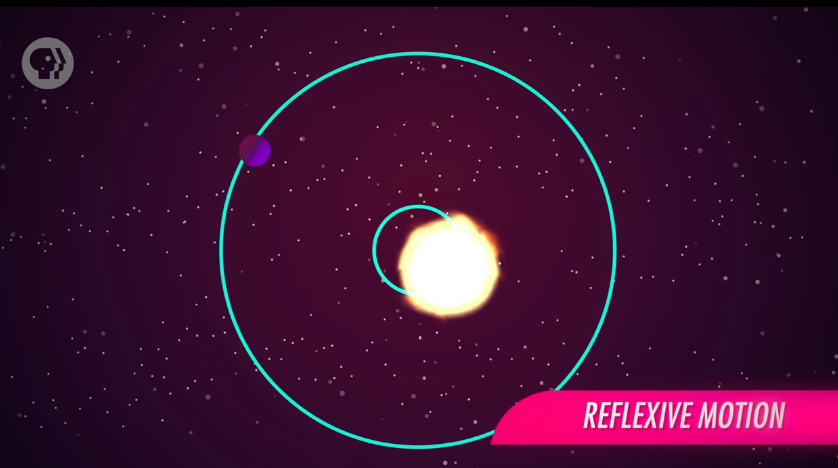
\includegraphics[width=0.40\textwidth]{Radial}
                    \caption{Documental: Exoplanets de Clash Course}
                \end{figure}

                El método de la velocidad radial se basa en el hecho de que una estrella no permanece completamente estacionaria
                cuando es orbitada por un planeta. Se mueve, aunque sea ligeramente, en un pequeño círculo o elipse,
                respondiendo al tirón gravitacional de su compañero más pequeño. Cuando se ven desde una distancia,
                estos movimientos leves afectan el espectro de luz normal de la estrella, o la firma de color.
                
                Si la estrella se está moviendo hacia el observador, entonces su espectro aparecerá ligeramente desplazado hacia
                el azul; si se está alejando, se desplazará hacia el rojo.
                \cite{wea6}
                
                
            \vspace{1em}
            \subsubsection{Transito}

                Este método detecta planetas distantes midiendo el minuto de atenuación de una estrella a medida que un
                planeta en órbita pasa entre ella y la Tierra. El paso de un planeta entre una estrella y la Tierra se
                llama un "tránsito". Si tal atenuación se detecta a intervalos regulares y dura un período de tiempo fijo,
                es muy probable que un planeta esté orbitando la estrella y pasando frente a ella una vez por cada período orbital.


                \begin{figure}[h]
                    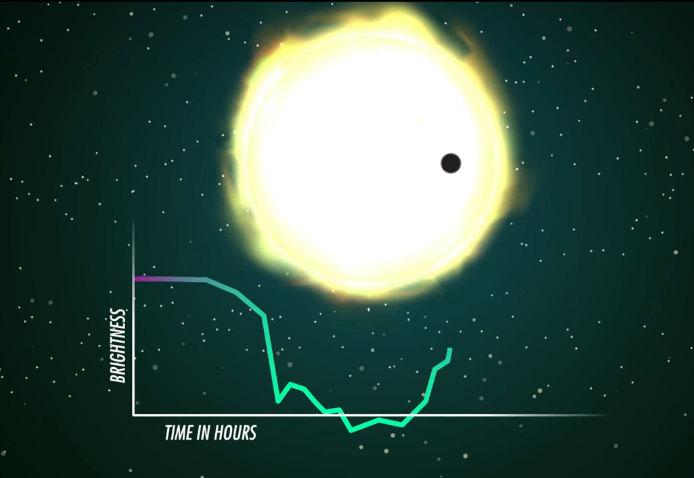
\includegraphics[width=0.40\textwidth]{Transit}
                    \caption{Documental: Exoplanets de Clash Course}
                \end{figure}

                La atenuación de una estrella durante el tránsito refleja directamente la relación de tamaño entre la estrella
                y el planeta: un pequeño planeta que transita una gran estrella creará solo una ligera atenuación, mientras
                que un gran planeta que transita una pequeña estrella tendrá un efecto más notable. El tamaño de la estrella
                anfitriona se puede conocer con una precisión considerable de su espectro, y la fotometría, por lo tanto,
                proporciona a los astrónomos una buena estimación del tamaño del planeta orbital, pero no de su masa.
                
                Esto hace que la fotometría sea un excelente complemento del método espectroscópico, que proporciona una estimación
                de la masa de un planeta, pero no su tamaño. Usando ambos métodos, combinando masa y tamaño, los científicos pueden
                calcular la densidad del planeta, un paso importante para evaluar su composición.
            
                \vspace{1em}
                \textbf{Análizar las atmósfera}

                A medida que el planeta se mueve frente a la estrella, su brillo disminuye. 
                Este planeta tiene una atmósfera que absorbe la luz azul y verde de manera eficiente
                mientras deja pasar la luz roja. Midiendo la disminución del brillo en diferentes longitudes 
                de onda, se puede obtener la transmitancia de la atmósfera dependiente de la longitud de onda.

        
        \vspace{1em}
        \subsection{Avances en este campo de investigación}
        
            \vspace{1em}
            \subsubsection{Kepler}

            \vspace{1em}
            \subsubsection{TESS}

            \vspace{1em}
            \subsubsection{Aportaciones de México}

                En México solo se ha descubierto un solo exoplaneta por parte del Instituto de Astronomía de la UNAM
                que desarrollaron su propio algoritmo, todo bajo el mando del doctor Jorge Cantú.

                Paso que el hallazgo no se realizó porque el trabajo era buscar exoplanetas, sino que fue por
                el desarrollo de una aplicación para hacer un ajuste de otros modelos astronómicos.

                Se empleó un algoritmo llamado “algoritmo genético asexual” (AGA) que regularmente tiene aplicaciones
                en áreas genéticas.

                Se probó el AGA para ver su funcionabilidad en la estrella 55 Cancri,
                de la cual se sabía que tenía cuatro planetas. Se aplicó el método y el resultado fue
                infalible, era el mismo con el que los otros científicos habían logrado su descubrimiento.

                Tiempo después, se aplicó a la observación de la estrella de Upsilon Andrómeda, en esta
                estrella se había confirmado la presencia de 3 planetas que orbitaban alrededor de Upsilon Andrómeda.
                
                El primero descubierto en 1997 y los otros dos en 1999, ambos por grupos de científicos estadunidenses,
                de la San Francisco State University y del Harvard-Smithsonian Center for Astrophysics.

                Pero AGA predijo cuatro, este cuarto planeta mejoraba bastante toda la información que tenián sobre
                el sistema, por lo que el grupo de Cantú publicó un paper con sus descubrimientos.
                \cite{wea4}
            
        \subsection{Análisis de los algoritmos utilizados}
                
            \vspace{1em}
            \subsubsection{Redes Neuronales}

                Las redes neuronales se basan en algunas ideas sobre cómo funcionan las neuronas en el cerebro,
                aunque creo que hay algunas diferencias significativas entre las redes neuronales informáticas y
                las redes neuronales en los organismos vivos.

                \begin{figure}[h]
                    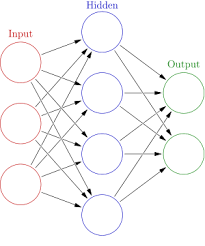
\includegraphics[width=0.25\textwidth]{redes}
                    \caption{Fuente: Wikicommons}
                \end{figure}

                En el aprendizaje automático, una red neuronal se inicializa para tener ciertas neurona
                conectadas de una manera particular. Cada neurona puede realizar un cálculo dado en su entrada y
                produce una salida, que puede ir a más neuronas.

                Ejecuta una entrada a través de la red y obtiene un resultado al final. Dependiendo de si el
                resultado se considera bueno o malo, los pesos de las conexiones entre las neuronas se ajustan
                (esto se realiza mediante un proceso denominado "propagación hacia atrás"). Usted ejecuta una
                gran cantidad de entradas y, según el resultado de cada ejecución, se ajustan los pesos, lo que
                afecta lo que sucederá en la siguiente ejecución.

                No es trivial, pero si puede configurar la red correctamente, el resultado es que la red puede
                aprender de manera efectiva a través del tiempo cómo producir resultados que se consideran buenos
                para una entrada determinada.

                Los éxitos modernos en el aprendizaje automático, como el AlphaGo de Deep Mind, dependen de la
                capacidad de utilizar recursos informáticos distribuidos extremadamente grandes para entrenar
                la red neuronal.


            \vspace{1em}
            \subsubsection{Algoritmos Geneticos}

                Es una técnica de optimización basada en los principios de la genética y la selección natural.
                Con frecuencia se utiliza para encontrar soluciones óptimas o casi óptimas para problemas difíciles
                que, de lo contrario, llevaría toda una vida resolverlos.
                
                Se usa frecuentemente para resolver problemas de optimización, en investigación y en aprendizaje automático.

                En estos, tenemos un grupo o una población de soluciones posibles para el problema dado.
                Estas soluciones luego se someten a recombinación y mutación (como en la genética natural),
                lo que produce nuevos individuos y el proceso se vuelve a repetir a lo largo de varias generaciones. 
                
                A cada individuo (o solución candidata) se le asigna un valor de adecuación
                (basado en su valor de función objetivo) y a los individuos más en forma se
                les da una mayor oportunidad de aparearse.

                \begin{figure}[h]
                    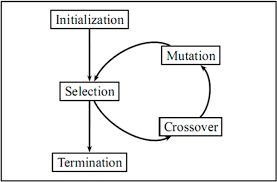
\includegraphics[width=0.30\textwidth]{genetic}
                    \caption{Fuente: Wikicommons}
                \end{figure}
                
                Esto está en línea con la Teoría Darwiniana de "Supervivencia del más apto".

                \cite{wea1}


    \begin{thebibliography}{1}

        \bibitem{wea1}
            I. A. Ruge, M. A. Alvis,
            \Quote{Aplicación de los algoritmos genéticos para el diseño de un controlador PID adaptativo},
            Tecnura, vol. 13,no. 25, p.p. 82,83 y 87, 2009. Disponible en:
            <http://www.redalyc.org/articulo.oa?id=257020617008>

        \bibitem{wea2}
            M. Gestal, et. al.,
            \Quote{Introducción a los algoritmos genéticos y programación
            genetica} , Universidad de Coruña, Coruña, 2010, ISBN: 978-84-9749-422-9

        \bibitem{wea3}
            A. Rodríguez-González, et. al., \Quote{Multi-component analysis
            of position-velocity cubes of the HH 34 Jet}, Astronomical
            Journal, vol. 143,no. 3, Febrero, 2012. Disponible
            en: <http://www.astroscu.unam.mx/apn6/PROCEEDINGS/B21-Rodriguez.pdf>

        \bibitem{wea4}
            J. Canto, S. Curiel and E. Martínez-Gómez.
            \Quote{
            A simple algorithm for optimization
            and model fitting: AGA (Asexual Genetic Algorithm)}, Astronomy
            \& Astrophysics, manuscript no. 1740ms, Aceptado, Mayo 31, 2008. Disponible:
            <https://www.aanda.org/articles/aa/pdf/2009/27/aa11740-09.pdf>

        \bibitem{wea5}
            J. Schneider, \Quote{Definition of Exoplanets and Brown Dwarfs} Handbook of Exoplanets, pp. 1–6, 2018.

        \bibitem{wea6}
            D. W. Latham, \Quote{Radial-Velocity Planets} Encyclopedia of Astrobiology, pp. 1400–1404, 2011.

        \bibitem{wea7}
            J. N. Winn, \Quote{Planet Occurrence: Doppler and Transit Surveys,} Handbook of Exoplanets, pp. 1–18, 2018.

        \bibitem{wea8}
            C. Kitchin, \Quote{Exoplanets and Exoplanetary Systems: Pasts and Futures} 
            Exoplanets Astronomers Universe, pp. 191–202, 2011.

    \end{thebibliography}

\end{document}